\documentclass{article}
\usepackage[margin=1.5in,a4paper]{geometry}
\usepackage[utf8]{inputenc}
\usepackage[
	backend=biber,
	style=numeric
]{biblatex}
\addbibresource{../bibliography.bib}
\usepackage[dvipsnames]{xcolor}
\usepackage{csquotes}
\usepackage{url}
\usepackage{graphicx}
\graphicspath{{./images/}}
\usepackage{booktabs}
\usepackage{hyperref}
\hypersetup{
	colorlinks=true,
	linkcolor=blue,
	urlcolor=blue,
	citecolor=blue,
}
\usepackage{comment}
\usepackage[font=footnotesize,labelfont=bf]{caption}


\title{Rethinking Model Architecture and Means of Delivery to get Unique Video Interation with Generative Neural Networks Online}
\date{\today}
\author{Josh Murr}

\begin{document}

\pagenumbering{gobble}
\maketitle
% \newpage
% \pagenumbering{arabic}
% \tableofcontents
% \newpage

\begin{abstract}
	% 250 Words
	This paper is about exploring the challenges and limitations of getting an experience like that of \textit{Learning to See} online; working on machines which do not have a powerful GPU and available to many more people.
\end{abstract}

\section{Introduction}
% 500 Words
% --- 568 WORDS ---
Machine Learning (ML) is a part of our everyday lives. For the technical among us it is currently easy enough to see the patterns in the outputs of these black-box systems; as the end of our sentence is predicted as we type, or an item we did not know we wanted is offered to us as we shop. There are however many non-technical users of ML systems who can only see the black-box, or perhaps nothing at all; as Arthur C. Clarke famously said \textit{``Any sufficiently advanced technology is indistinguishable from magic.''}\cite{toffler_1972} It is often the case that exciting new technologies are adopted by artists as readily as industry because the gallery provides a unique environment to present back the to the user one of these black-boxes in a drastically different context. Artists such as Mario Klingemann\cite{mario_klingemann}, Terence Broad\cite{terry_broad} or Anna Ridler\cite{anna_ridler} are all excellent examples of artists who have done just this; delivering the \textit{medium as the message}.

\begin{figure}
	\centering
	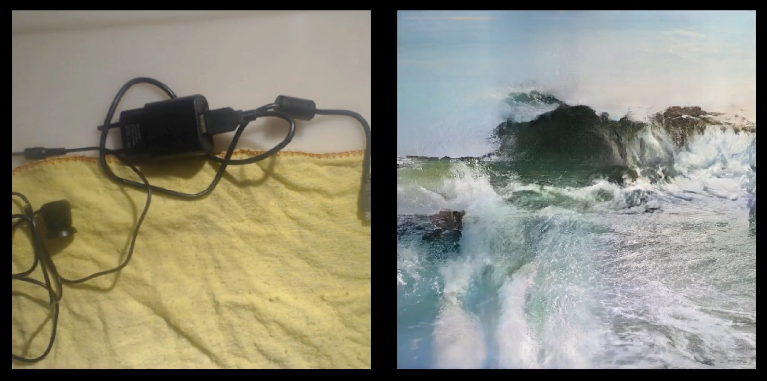
\includegraphics[scale=0.3]{lts_still}
	\caption{A frame from Learning to See using a model trained on ocean waves. --- \copyright Memo Akten,2017}
\end{figure}

\textit{Learning to See} by Memo Akten\cite{lts_memo} is another example, but unique in its own way in that it gives the user an interactive experience of the artwork; an immediate image translation of arbitrary objects on a tabletop to a rich image of waves crashing, the night sky or everchanging flowers. The user is able to manipulate the input data as they move the objects on the table and witness how the model interprets this data to produce an output image projected in front of them. Although the model still exists as a black box, being able to see how input-affects-output in real time is extremely powerful.


Witnessing the relationship between input and output is in many ways more vital to understanding the function of a Neural Network (NN) than understanding what a neuron is and how backpropagation works. The role of the artist is important here as these artworks have done a huge amount to shed light on dataset bias\cite{crawford_paglen_2019}, stimulate conversation about ownership and copyright\cite{romano_2016} and show both the capabilities of ML systems \textit{and} the limitations. It is therefore of great importance to make these stimulating artworks accessible to as many people as possible, which is not as simple as it might seem.

Unfortunately the gallery in itself is a black box to many, entry restricted by a fee or simply by the location of the gallery. Moving such interactive experiences online is a clear next step as once something is online it is immediately available to anyone with an internet connection --- this then poses numerous more challenges. Even a modestly sized NN can contain many millions of parameters. Modern computers are able to perform millions of floating point operations per second (FLOPS) but advances in ML research have shown that \textit{deeper} models and more data produces better results\cite{2005.14165}; as such, without expensive hardware accelleration from discrete graphics processing units (GPU) or even more modern tensor processing units (TPU), an average modern computer cannot crunch the numbers needed to run a large, deep NN\@. Even if one \textit{could} perform the necessary FLOPS, storing this number of parameters can take up gigabytes of memory and so downloading the weights and biases of a pre-trained model can be a time consuming process detracting from the real-time focus.

This paper aims to explore each of these challenges and to look at each through the perspective of the artworks previously described with the aim of getting a piece like \textit{Learning to See} online and useable by most users.


\section{Background Context}
% 500-1000 Words
% --- 891 WORDS ---

Getting NNs working online and on the clients machine is not a new thing and with modern CPUs it has certainly been shown possible to train and run a simple enough model in the browser on a modest computer\cite{karparthy_conjs_2016, brainjs, synaptic, mind, kerasjs} and many tools exist which aim to visualise the architecture of a model and show the training process\cite{broad_cnn_vis_2016, tensorflow_playground, 1704.01942}. Such tools are invaluable as learning resources for those dedicated to learning about machine learning. However they are often tailored to that use case expecting the user to have higher motivation for understanding what is going on than the average online `passer-by'.

There is an increasing number of tools available online which use an interactive machine learning approach allowing the user to retrain a model in real-time to create unique interactions of the users specification\cite{magenta, mimic, teachablemachines}. Again this is valuable work and useful to many, but often requires active engagement from the user even if the user-interaction is spoon-fed to them.

\textit{Learning to See} provides an instinctive way for the user to interact with machine learning, avoiding technical terms or a prerequisite knowledge which is simply not seen online (at the time of writing). This is largely down to the issues described above, and these are especially applicable to image generative models which will be discussed further below.

\textit{Learning to See} is an adaptation of the Pix2Pix model\cite{1611.07004} which is a Conditional Generative Adversarial Network (cGAN)\cite{1701.00160}. Unlike a conventional GAN\cite{1406.2661}, a cGAN takes in two data samples as input, in the case of the Pix2Pix model it is a \textit{target} image and an \textit{input} image. Pix2Pix also learns a structured loss which means it is able to penalize any possible structure that differs between output and target\cite{1611.07004}. This model architecture is extremely flexible and has been shown to be useful for many use cases as detailed in the original paper. However neither the original Pix2Pix paper or \textit{Learning to See} had an incentive to create a small model; a good result is simply a sharp image with a predictable output from a given input. As stated by the Pix2Pix authors measuring the results of an image generating GAN is an open issue\cite{1606.03498, 1611.07004} and in an artistic context quatifiying the outcome is largely pointless. A good result is one which delivers the message of the artist, thus if a meaningful interaction can be acheived then perhaps some sacrifices can be made to improve the speed and reduce the size of the model.

It is worth noting that other generative models of similar architecture to Pix2Pix have been developed since, notably CycleGAN\cite{1703.10593} and GauGAN\cite{1903.07291}. However these models are also significantly more complex and did not seem conducive to a lightweight and performant system with the given requirements. Image generative models are notoriously unstable in training, intuition (and Jonathan Hui) notes that it is easier to recognise an image than it is to create one\cite{hard_to_train_gans}. Therefore traditional NN compression\cite{2006.03669} is often unsuited to GANs. There has been work in GAN compression which has yielded impressive results, but it is a quite esoteric, unconventional compression involving programatically finding alternate model architectures with nerual architecture search (NAS) and teacher--student model pairing to distill knowledge into a smaller architecture\cite{2003.08936}. Simplicity was the first port-of-call for this work thus methods shown in the aforementioned works remain untested in this context for now.

Designing and training a NN is of course not limited to the big name ML frameworks like Tensorflow\cite{tf} or PyTorch\cite{pytorch}, but given the modular nature of a NN and the want in most cases to utilise the GPU for faster training and inference, it is no surprise that a limited number of ML frameworks have become the goto to create and iterate on a novel ML model and to take care of interfacing with a highly optimized backend and the GPU at a lower level. Tensorflow offers a relatively full end-to-end pipeline from designing and training a model in Python, to saving and converting a model into something can be run in the browser using TensorflowJS\cite{tfjs}. A trained model is simply a collection of weights and biases and to use this model on a different device or context, these weights and biases need to be loaded into a model of the same architecture as was used to train the model. The pipeline from training-to-browser is largely about keeping data structures in order and consistent such that the next process knows how to work with it. As part of the process Tensorflow as developed the TensorflowJS Converter\cite{tfjs_converter} which creates a \verb|model.json| file which is the blueprints of the model, and a series of binary files which hold the weights. The pipeline developed by the team at Google behind Tensorflow is great acheivement, as ML model design as a broad field and needs to be flexible; catering for this flexibility is no easy task. The framework needs to interpret and reimplement a model consisting of many layers and potentially millions of parameters in an entirely new context for it work in the browser. This felxibility comes at a performance cost however which can be observed in a naive implementation of \textit{Learning to See} which will be covered in more detail later. In order to recreate a model based on the provided \verb|model.json| file, seperate programs in the chosen backend (WebGL, WebAssembly, WebGPU, etc.) are created to take care of specific tasks such as 2D convolutions, batchnorm, max pooling etc. Moving data through the computational graph is now the difficult part as each of these stages exists as a discrete routine which performs efficient calculations, but getting the data out of the GPU to pass on to the next program comes at a great performance cost and increases latency of the overall system, particularly with web technologies\cite{optimizing_webgl}.

There exists nothing even similar to \textit{Learning to See} in the catalog of examples provided by TensrflowJS --- ie a model which takes video as input and produces video as output. Thus the uniqueness of this use case has yielded a number of hurdles to overcome to acheive something usable on the web for \textit{most users} (users with a reasonably modern laptop, produced in the past 5 years).


\section{Method}
% 500-750 words - how you will approach the problem
% (use well understood methods and don’t roll your own)
% mixed methods fine (quantitative - data and qualitative - surveys, viewpoints)
% --- 892 WORDS ---
TensorflowJS is currently the most developed framework for deploying models in the browser so working with the Tensorflow pipeline made the most sense. The model for this work was based on the Tensorflow implementation\cite{tf_p2p} and adjusted according to the \textit{Learning to See} paper: the input and target images are the same, only the input goes through a series of augmentations, details of which can be found in the original paper\cite{2003.00902}.

The data augmentation requires the generator to take a single channel input. Augmenting the dataset at runtime during training makes forming a dataset very easy as in reality a full dataset is simply a directory of many similar images. As stated earlier, evaluating the model quantitatively by some distance metric has been shown to be of little use, and particularly in this case the quality of the outcome can only really be measured by how well it performs when interacted with. Thus the common process of splitting a dataset into \textit{training} and \textit{testing} data at a 4:1 split was not as important; however approximately 5\% of the dataset was reserved for testing after training for visual inspection.

\begin{figure}
	\centering
	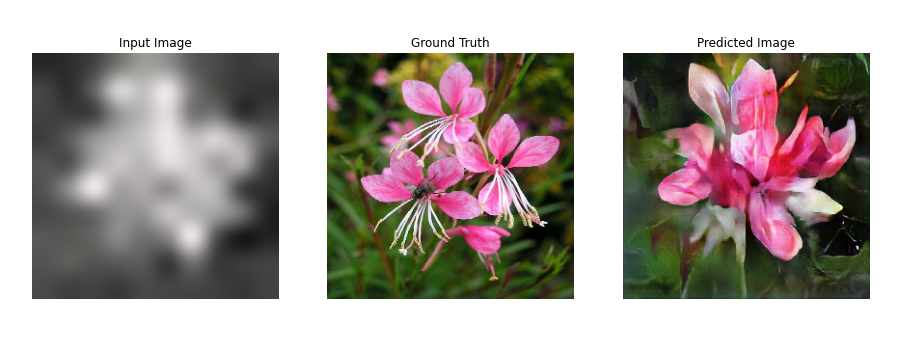
\includegraphics[width=\textwidth]{250_epochs}
	\caption{A caption.}
\end{figure}

It was found that for a model that takes an input image size of 256$\times$256 pixels and produces an output of the same size, a dataset of 800--1000 images uniformly shuffled with a batch size of 4, trained for 200--250 epochs was sufficient to produce \textit{interesting} results --- in this case \textit{interesting} means: varied enough to provide unique experiences whilst producing a output which is representative of the input data. The models were trained on a NVIDIA Quadro RTX 6000 with 24GB memory locally, or a Tesla P100-PCIE with 16GB memory using Google Colab. In either case a usable model will train in a few hours allowing for a relatively quick development cycle. More details on the training process and some tools developed to make the process easy and fast in the appendix.

The Pix2Pix generator is an Autoencoder similar to the ``U-Net'' architecture\cite{1505.04597} but differs in some key ways, and we offer some further changes to drastically reduce the size. The generator consists of 8 2D convolution layers downsampling the input data in width and height, and 7 transpose convolutions upsampling the data back to original size. Each layer is batchnormalized\cite{1502.03167} apart from the first, and layers 8--10 have dropout\cite{JMLR:v15:srivastava14a} applied at a rate of 50\%. The Pix2Pix architecture includes no avg- or max-pooling as all filter kernels are 4$\times$4 and a stride of 2 is used. This has the effect of downsampling the layer input by half in width and height, thus circumventing the need for any kind of pooling, otherwise known as an \textit{all convolutional net}\cite{1412.6806}. The difference proposed in this work is to greatly reduce the number of filters used in each layer. The majority of trainable parameters are found in the middle of the generator as a result of the structure described. By reducing the number of filters in each layer by up to a factor 8, very usable results were obtained whilst drastically reducing the model size.

\begin{small}
	\begin{center}
		\begin{tabular}{p{2cm} p{2cm} p{2cm}}
			\toprule
			Generator Layer & Pix2Pix Filters & Our Filters \\
			\midrule
			1               & 64              & 8           \\
			2               & 128             & 16          \\
			3               & 256             & 32          \\
			4               & 512             & 64          \\
			5               & 512             & 128         \\
			6               & 512             & 256         \\
			7               & 512             & 512         \\
			8               & 512             & 512         \\
			9               & 512             & 512         \\
			10              & 512             & 256         \\
			11              & 512             & 128         \\
			12              & 512             & 64          \\
			13              & 512             & 32          \\
			14              & 256             & 16          \\
			15              & 128             & 8           \\
			\bottomrule
		\end{tabular}
	\end{center}
\end{small}

Once a model is trained, it is saved using the \verb|HDF5| format (\verb|.h5|) and converted using the TensorflowJS Converter. The Converter provides options for compressing the model of varying levels of severity. It was found that the compression of the model:

\begin{enumerate}
	\item Does a great deal to reduce the size (in memory) of the model.
	\item Does very little to improve performance in inference.
	\item Does very little to affect the output of the model.
\end{enumerate}

Therefore the highest compression of \verb|uint8_affine_quantize| can be used to reduce the size by an order of magnitude, while maintaining only a very slightly compromised output.

Finally, a bespoke WebGL wrapper consisting of a number of shader programs was created to handle the input data (pre-augmentation to match that in training) and the output data to render the image to the screen as video. It was found that the image handling capabilities of TensorflowJS seem to be tailored to static images. In inference, the data is of the \textit{tensor} data structure and is transformed and manipulated by the model, but at each iteration of the draw cycle a frame of video must be preprocessed and then converted into a format which can be digested by the model, and then the output of the model must be converted back into a data structure which the browser can handle to display as an image, or in our case, video. The internal computation at inference is handled by WebGL shader programs compiled by TensorflowJS, but the input/output was a rather slow process of converting the tensor data back to pixels value-by-value. The input shader programs take data from the webcam as a 16$\times$16 image and scales it up to 256$\times$256 while applying three gaussian blurs --- slightly different to the training process but the effect is the same. The output of the model is passed into a very simple shader program as a 32 bit floating point RGB texture and is rendered to a canvas element in the browser.

\begin{comment}
It can be observed in the stack trace (using the developer tools of most modern browsers, in this case Firefox and Chrome were used) that TensorflowJS is still having to do a lot of the working moving data around and reshaping data in Javascript, while the heavy computation is deferred to shader programs. This moving data around comes at a great cost which is felt particualrly in the case of video based interaction. As a slight aside, a `pure' WebGL Autoencoder of the same stucture as the Pix2Pix generator was created simply to perform the same number of calculations in the same fashion to compare performance, and to give a glimpse into a novel approach to machine learning online which is perhaps more streamlined.
\end{comment}

\section{Results}
% 500-750 words
% -- 389 WORDS ---
A test-bed was created with the aforementioned processes to test three sizes of model. The project is currently online at \url{https://learning-to-learn-to-see.netlify.app/}. % In the table below \textit{Avg Step Time} is the time taken to create a new frame to output which includes pre-processing and post-processing via the custom WebGL wrapper.

\begin{figure}
	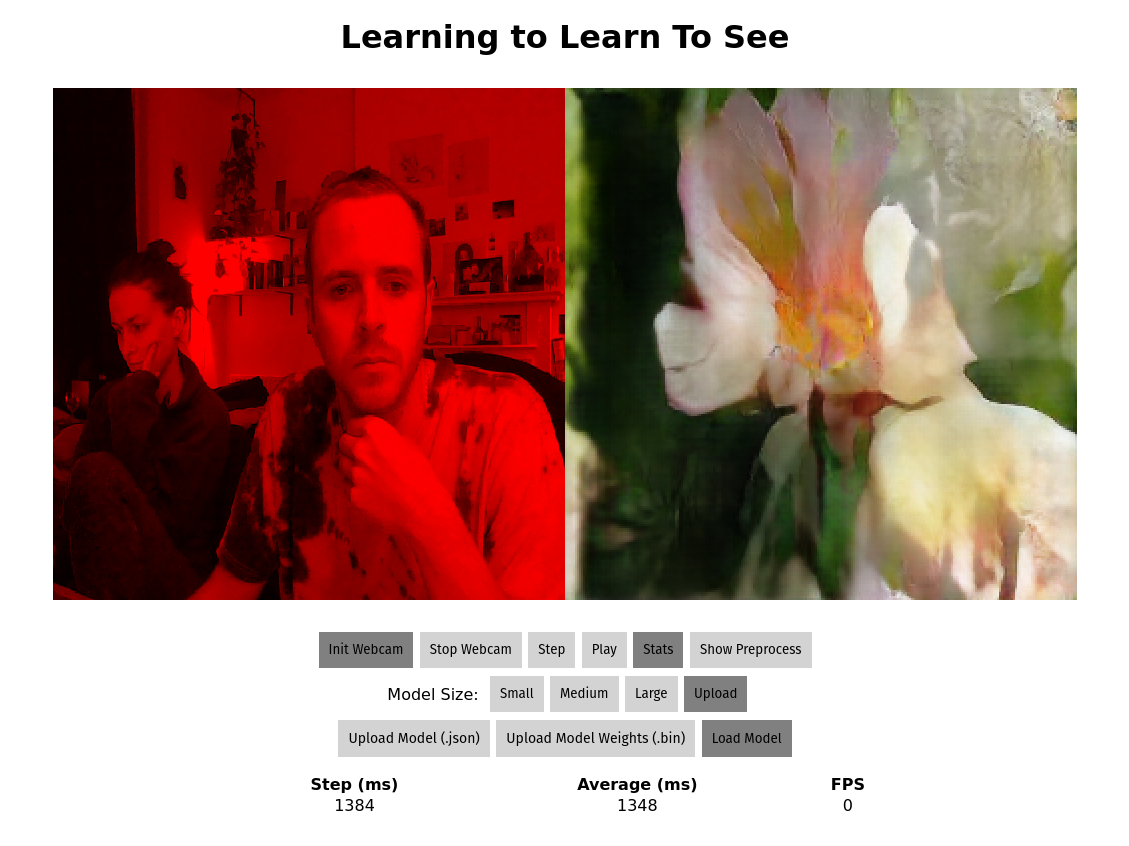
\includegraphics[width=8cm]{ltlts_online}
	\centering
\end{figure}


\begin{small}
	\begin{center}
		\begin{tabular}{p{1.5cm} p{1.5cm} p{1.5cm} p{1.5cm} p{1.5cm} p{1.5cm}}
			\toprule
			       & HDF5 Size (mb) & Uint8 Compressed Size (mb) & Compression & Total Parameters & Upload Time (s) \\
			\midrule
			Small  & 25.3           & 6.3                        & 25.2\%      & 6,297,491        & 8.3             \\
			Medium & 67.3           & 16.9                       & 25.0\%      & 16,786,211       & 9.9             \\
			Large  & 217.8          & 54.5                       & 25.0\%      & 54,423,811       & 27.5            \\
			\bottomrule
		\end{tabular}
	\end{center}
\end{small}

%Small  & 25323104           & 6365943 
%Medium & 67280248           & 16852241
%Large  & 217835560          & 54484213


As already stated, the focus was on finding a sufficiently responsive interaction for the user while maintaining enough variety in the output to maintain engagement. The target audience is someone with a relatively modern computer and not necessarily someone with a computer with a high specification GPU. For testing the user is able to download a model size at their choosing or upload their own, and different statistics are displayed.

In the table below \textit{D-GPU} means \textit{Discrete-GPU} and \textit{I-GPU} means \textit{Integrated-GPU}. \textit{FPS} is rounded to the nearest number.

\begin{small}
	\begin{center}
		\begin{tabular}{p{5cm} p{1.5cm} p{1.5cm} p{1.5cm}}
			\toprule
			\multicolumn{4}{c}{Performance (FPS) on Various Computers} \\
			\toprule
			Machine                     & Small & Medium & Large       \\
			\midrule
			System76 Laptop 2020, D-GPU & TODO  & TODO   & TODO        \\
			System76 Laptop 2020, I-GPU & 26    & 12     & 0           \\
			Macbook Pro 2017, D-GPU     & 40    & 27     & 0           \\
			Macbook Pro 2017, I-GPU     & 26    & 14     & 0           \\
			Macbook Pro 2020, I-GPU     & 25    & 15     & 1           \\
			Macbook Pro 2015, I-GPU     & 30    & 18     & 0           \\
			MSI Laptop 2016, I-GPU      & 18    & 12     & 1           \\
			Pixel 3A Phone              & 3     & -      & -           \\
			Samsung Phone               & 4     & -      & -           \\
			\bottomrule
		\end{tabular}
	\end{center}
\end{small}

In general the results are very promising. The average frame rate on an integrated GPU is $\sim$14FPS which suggests that the average `everyday' computer will be able to run the \textit{medium} sized model at a useable speed. However a good result in our case in more dependent on the quality of the interaction.

It can be observed that models trained with fewer parameters struggle to generalise. The \textit{102 Category Flower Dataset}\cite{flowers_dataset} has proven to be a useful dataset for testing as it is quite varied; the subject is not always centered in the image, the colours vary drastically and there is great variation in tone and texture throughout. A full sized \textit{large} model is capable of capturing a lot of this texture, however with fewer filters in the smaller models, artefacts of the kernels themselves often appear in the output, as seen below.

\begin{figure}[h]
	\centering
	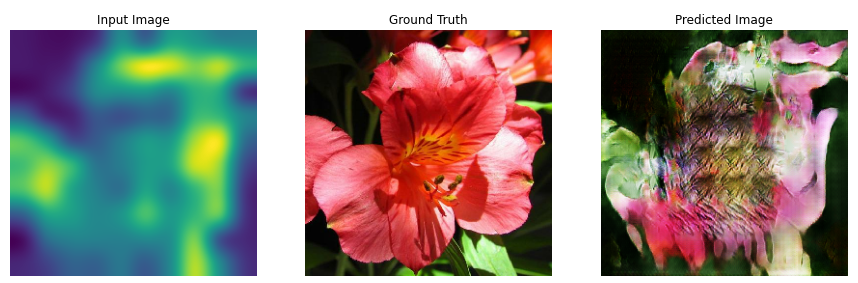
\includegraphics[scale=0.4]{artefacts}
	\caption{A caption.}
\end{figure}

In training the model is attempting to learn a mapping from a blurry greyscale image to a 3-channel, well defined image. As a user interacts using the online platform one can quickly see the effects of bright or dark areas, as in such an abstract input, the model appears to associate these bright spots with key areas on interest in the output.

With all this in mind one can train a model with a less varied dataset (such as daytime clouds) which still produces compelling results even in the smallest model as the model needs to generalise less. A dataset produced from a timelapse of the Aurora Borealis was used for the smallest model. The smallest model does not produce particularly exciting results, but still does a good job of illustrating the relationship between input and output, and has even been shown to work on mobile devices.

\begin{comment}
The aforementioned `pure' WebGL Autoencoder is a scalable CNN framework which holds the core functionality to perform the forward pass of an \textit{all convolutional} network, such as that of the Pix2Pix generator.
\end{comment}

\section{Discussion}
% As long as you can cope with
The adoption of ML research into the art world offers a reframing of the application of ML research, which in turn reframes the approach to research itself. The U-Net style all convolutional network used for the generator in the Pix2Pix model is a particularly graceful NN which at its core is \textit{only} a series 2D convolutions (omitting batchnormalisation and skip connections). This work shows that the network itself need not be very large to still produce results which, to the scientific community may not be progressive or impressive, but to get this kind of work in any way to more people opens up many possibilities. As stated, if this work reaches and excites people who previously saw generative ML as off limits, then it is considered a success. Beyond that this work could lead to the development even more artistic tools in the same way that ML5\cite{ml5}, RunwayML\cite{runway} and Wekinator\cite{wekinator} have become tools for experimentation among artists and creators.


\section{Conclusion}
% Sum up what you have learned and where we should go next

%\nocite{*} % Include all citations


\medskip
\printbibliography

\appendix
\section{Training Process}
Some text that will be the appendix.

\end{document}
